% Source: fixed PDF source-relative page 2 (printed page 307), Q20.
% Solid/hidden edges and midpoint E on OC follow the source geometry diagram.
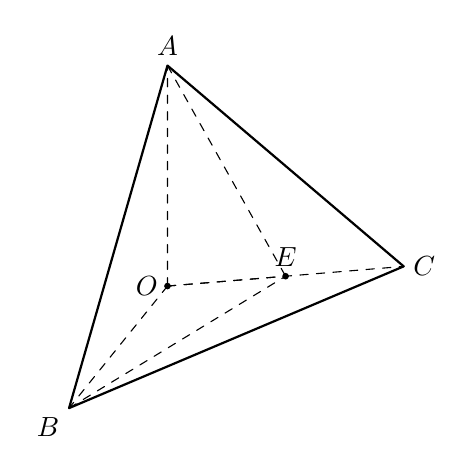
\begin{tikzpicture}[line cap=round,line join=round]
  \coordinate (A) at (0,2.8);
  \coordinate (B) at (-1.25,-1.55);
  \coordinate (C) at (3.0,0.25);
  \coordinate (O) at (0,0);
  \coordinate (E) at (1.5,0.125);
  % Visible boundary edges
  \draw[thick] (A)--(B)--(C)--cycle;
  \draw[dashed] (O)--(A) (O)--(B) (O)--(C);
  % Hidden interior edges in the printed view
  \draw[dashed] (O)--(E) (A)--(E) (B)--(E);
  \fill (O) circle[radius=1.2pt];
  \fill (E) circle[radius=1.2pt];
  \node[above] at (A) {$A$};
  \node[below left] at (B) {$B$};
  \node[right] at (C) {$C$};
  \node[left] at (O) {$O$};
  \node[above] at (E) {$E$};
\end{tikzpicture}
